
\section{Clustered Objects}
\label{sect:ClusteredObjects}

\subsection{Mass Fractal
\cite{Sorensen1999,Sorensen1992,Hurd1988,Lin1989,Lin1990,Lin1990a}}
\label{sect:MassFractal}
\hspace{1pt} \\

\begin{figure}[htb]
\begin{center}
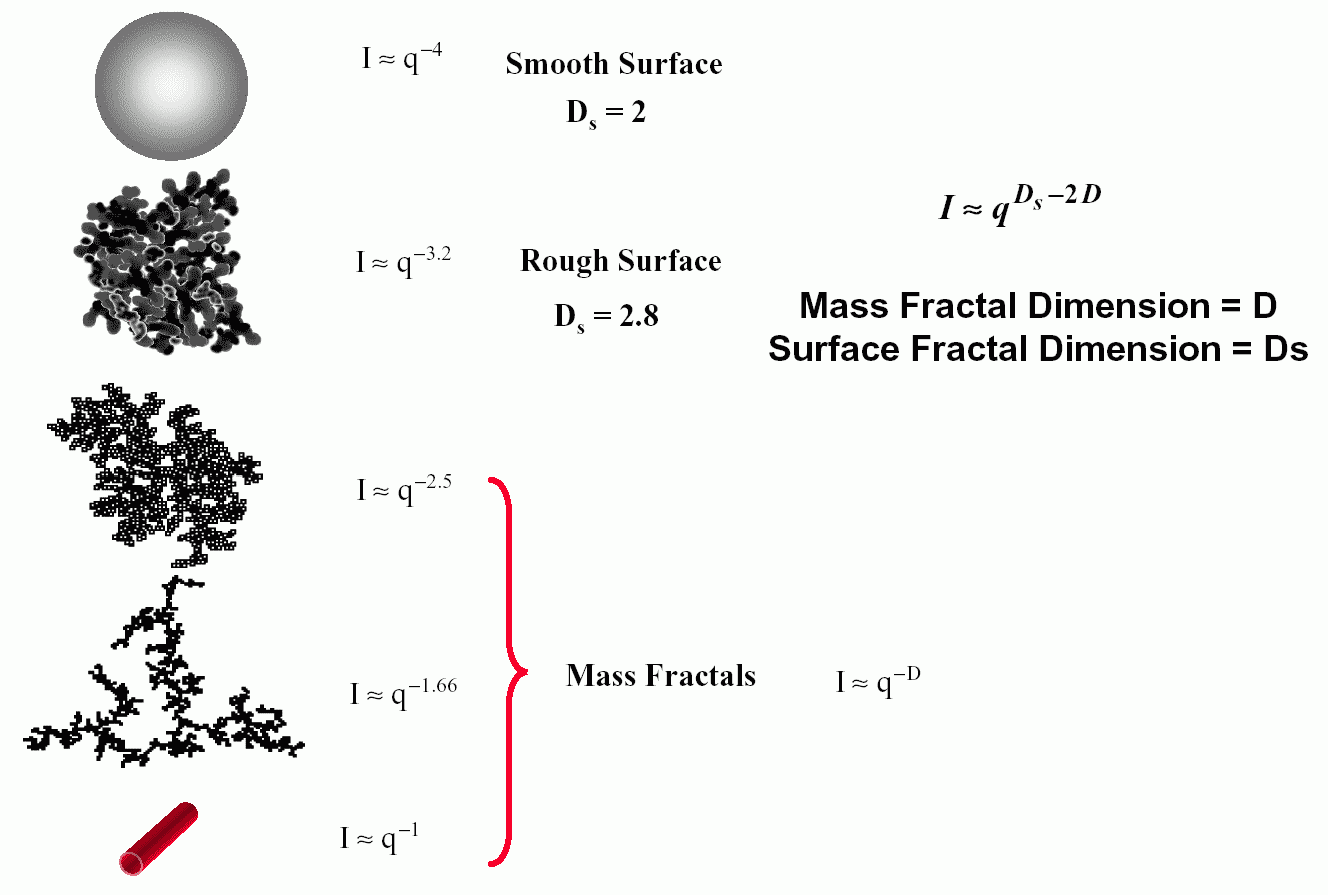
\includegraphics[width=0.9\textwidth,height=0.60665\textwidth]{../images/form_factor/cluster/fractaldimension.png}
\end{center}
\caption{} \label{fractaldimension}
\end{figure}

Aggregates and clusters often have a fractal morphology. These self-similar clusters are well
described by
\begin{align}
N=k_0(R_g/r_0)^D
\end{align}
where $N$ is the number of primary particles or monomers in the aggregate,
$k_0$ is a constant of order unity, $R_g$ is the radius of gyration of the aggregate,
$r_0$ is the monomer radius, and $D$ is the fractal dimension.

The scattering function and the density autocorrelation function
of the aggregate are Fourier transform pairs; thus
\begin{align}
I(q)=4\pi \int_0^\infty \, g(r)\, r^2\, \frac{\sin(qr)}{qr}\, dr
\label{eq:aggregateSQ}
\end{align}
For a fractal aggregate the autocorrelation function has the
form
\begin{align}
g(r) \sim r^{D-d} h(r,\xi)
\label{eq:aggregate_g(r)}
\end{align}
Here $D$ is the fractal dimension, $d$ the spatial dimension, and
$\xi$ a measure of the linear size of the aggregate proportional to
the radius of gyration $R_g$. The function $h(r,\xi)$ is the cutoff
function describing the perimeter of the aggregate. Its properties
are that $h(r,\xi) \simeq 1$ for $r/\xi \lesssim 1$, but for large
$r/\xi$ it falls off faster than any power law.

\noindent

\begin{table}[htb]
\caption{Scattering functions $I(q)$ for different cutoff functions
$h(r,\xi)$.
\label{tab:SQ_cutuofffunctions}}
\begin{tabular}{|c|c|c|c|c|}
  \hline
  & & & & \\[-2mm]
  % after \\: \hline or \cline{col1-col2} \cline{col3-col4} ...
  {\tt SASfit}-name & $h(r,\xi)$    & $\xi^2$   & $I(q)$    & Ref. \\
  & & & & \\[-2mm]
  \hline
  \hline
  & & & & \\[-2mm]
   {\tt \scriptsize Fischer-Burford}&  $\scriptstyle \text{ca. } \exp\left[-\tfrac{r}{\xi}\right]$  & $\scriptstyle R_g^2/3$ & $\scriptstyle \left(1+\frac{2}{3D}q^2R_g^2\right)^{-D/2}$ &  \\[3mm]
   {\tt \scriptsize MassFractExp}   & $\scriptstyle \exp\left[-\tfrac{r}{\xi}\right]$          & $\frac{2R_g^2}{D(D+1)}$ & $\scriptstyle \frac{\sin\left[(D-1)\arctan(q\xi)\right]}{(D-1)q\xi(1+q^2\xi^2)^{(D-1)/2}}$ &  \\[3mm]
   {\tt \scriptsize MassFractGauss} & $\scriptstyle \exp\left[-\left(\tfrac{r}{\xi}\right)^2\right]$ & $\frac{4R_g^2}{D}$ & $\scriptstyle e^{-\frac{q^2R_g^2}{D}} {}_1F_1\left[\frac{3-D}{2},\frac{3}{2},\frac{q^2R_g^2}{D}\right]$ &  \\[3mm]
   $\text{\tt \scriptsize Aggregate}\atop \text{\tt (Exp(-x$\hat~$a) Cut-Off)}$ & $\scriptstyle \exp\left[-\left(\tfrac{r}{\xi}\right)^\alpha\right]$ & --- & numerical &  \\[3mm]
   $\text{\tt \scriptsize Aggregate}\atop \text{\tt (OverlapSph Cut-Off)}$ & $ \scriptstyle
                                                    \begin{cases}\scriptstyle
                                                        \left(1+\tfrac{r}{4\xi}\right) \left(1-\tfrac{r}{2\xi}\right)^2 ,&  \scriptstyle r<2\xi\\
                                                        \scriptstyle 0 ,&  \scriptstyle r\geq 2\xi
                                                  \end{cases}$ & $\scriptstyle\frac{(D+2)(D+5)}{2D(D+1)}R_g^2$ & numerical &  \\[3mm]
   {\tt \scriptsize DLCAggregate} & --- & --- & $\scriptstyle \left[1+{\displaystyle \sum_{\scriptstyle s=1}^{\scriptstyle 4}}C_s(qR_g)^{2s}\right]^{-D/8}$ &  \\
                                          & & & $\scriptstyle C_1=\frac{8}{3}D, \, C_2=2.5$ & \\
                                          & & & $\scriptstyle C_3=-1.52, \, C_4=1.02$ & \\[3mm]
   {\tt \scriptsize RLCAggregate} & --- & --- & $\scriptstyle C_1=\frac{8}{3}D, \, C_2=3.13$ & \\
                                          & & & $\scriptstyle C_3=-2.58, \, C_4=0.95$ & \\[3mm]
  \hline
\end{tabular}
\end{table}


\begin{figure}[htb]
\begin{center}
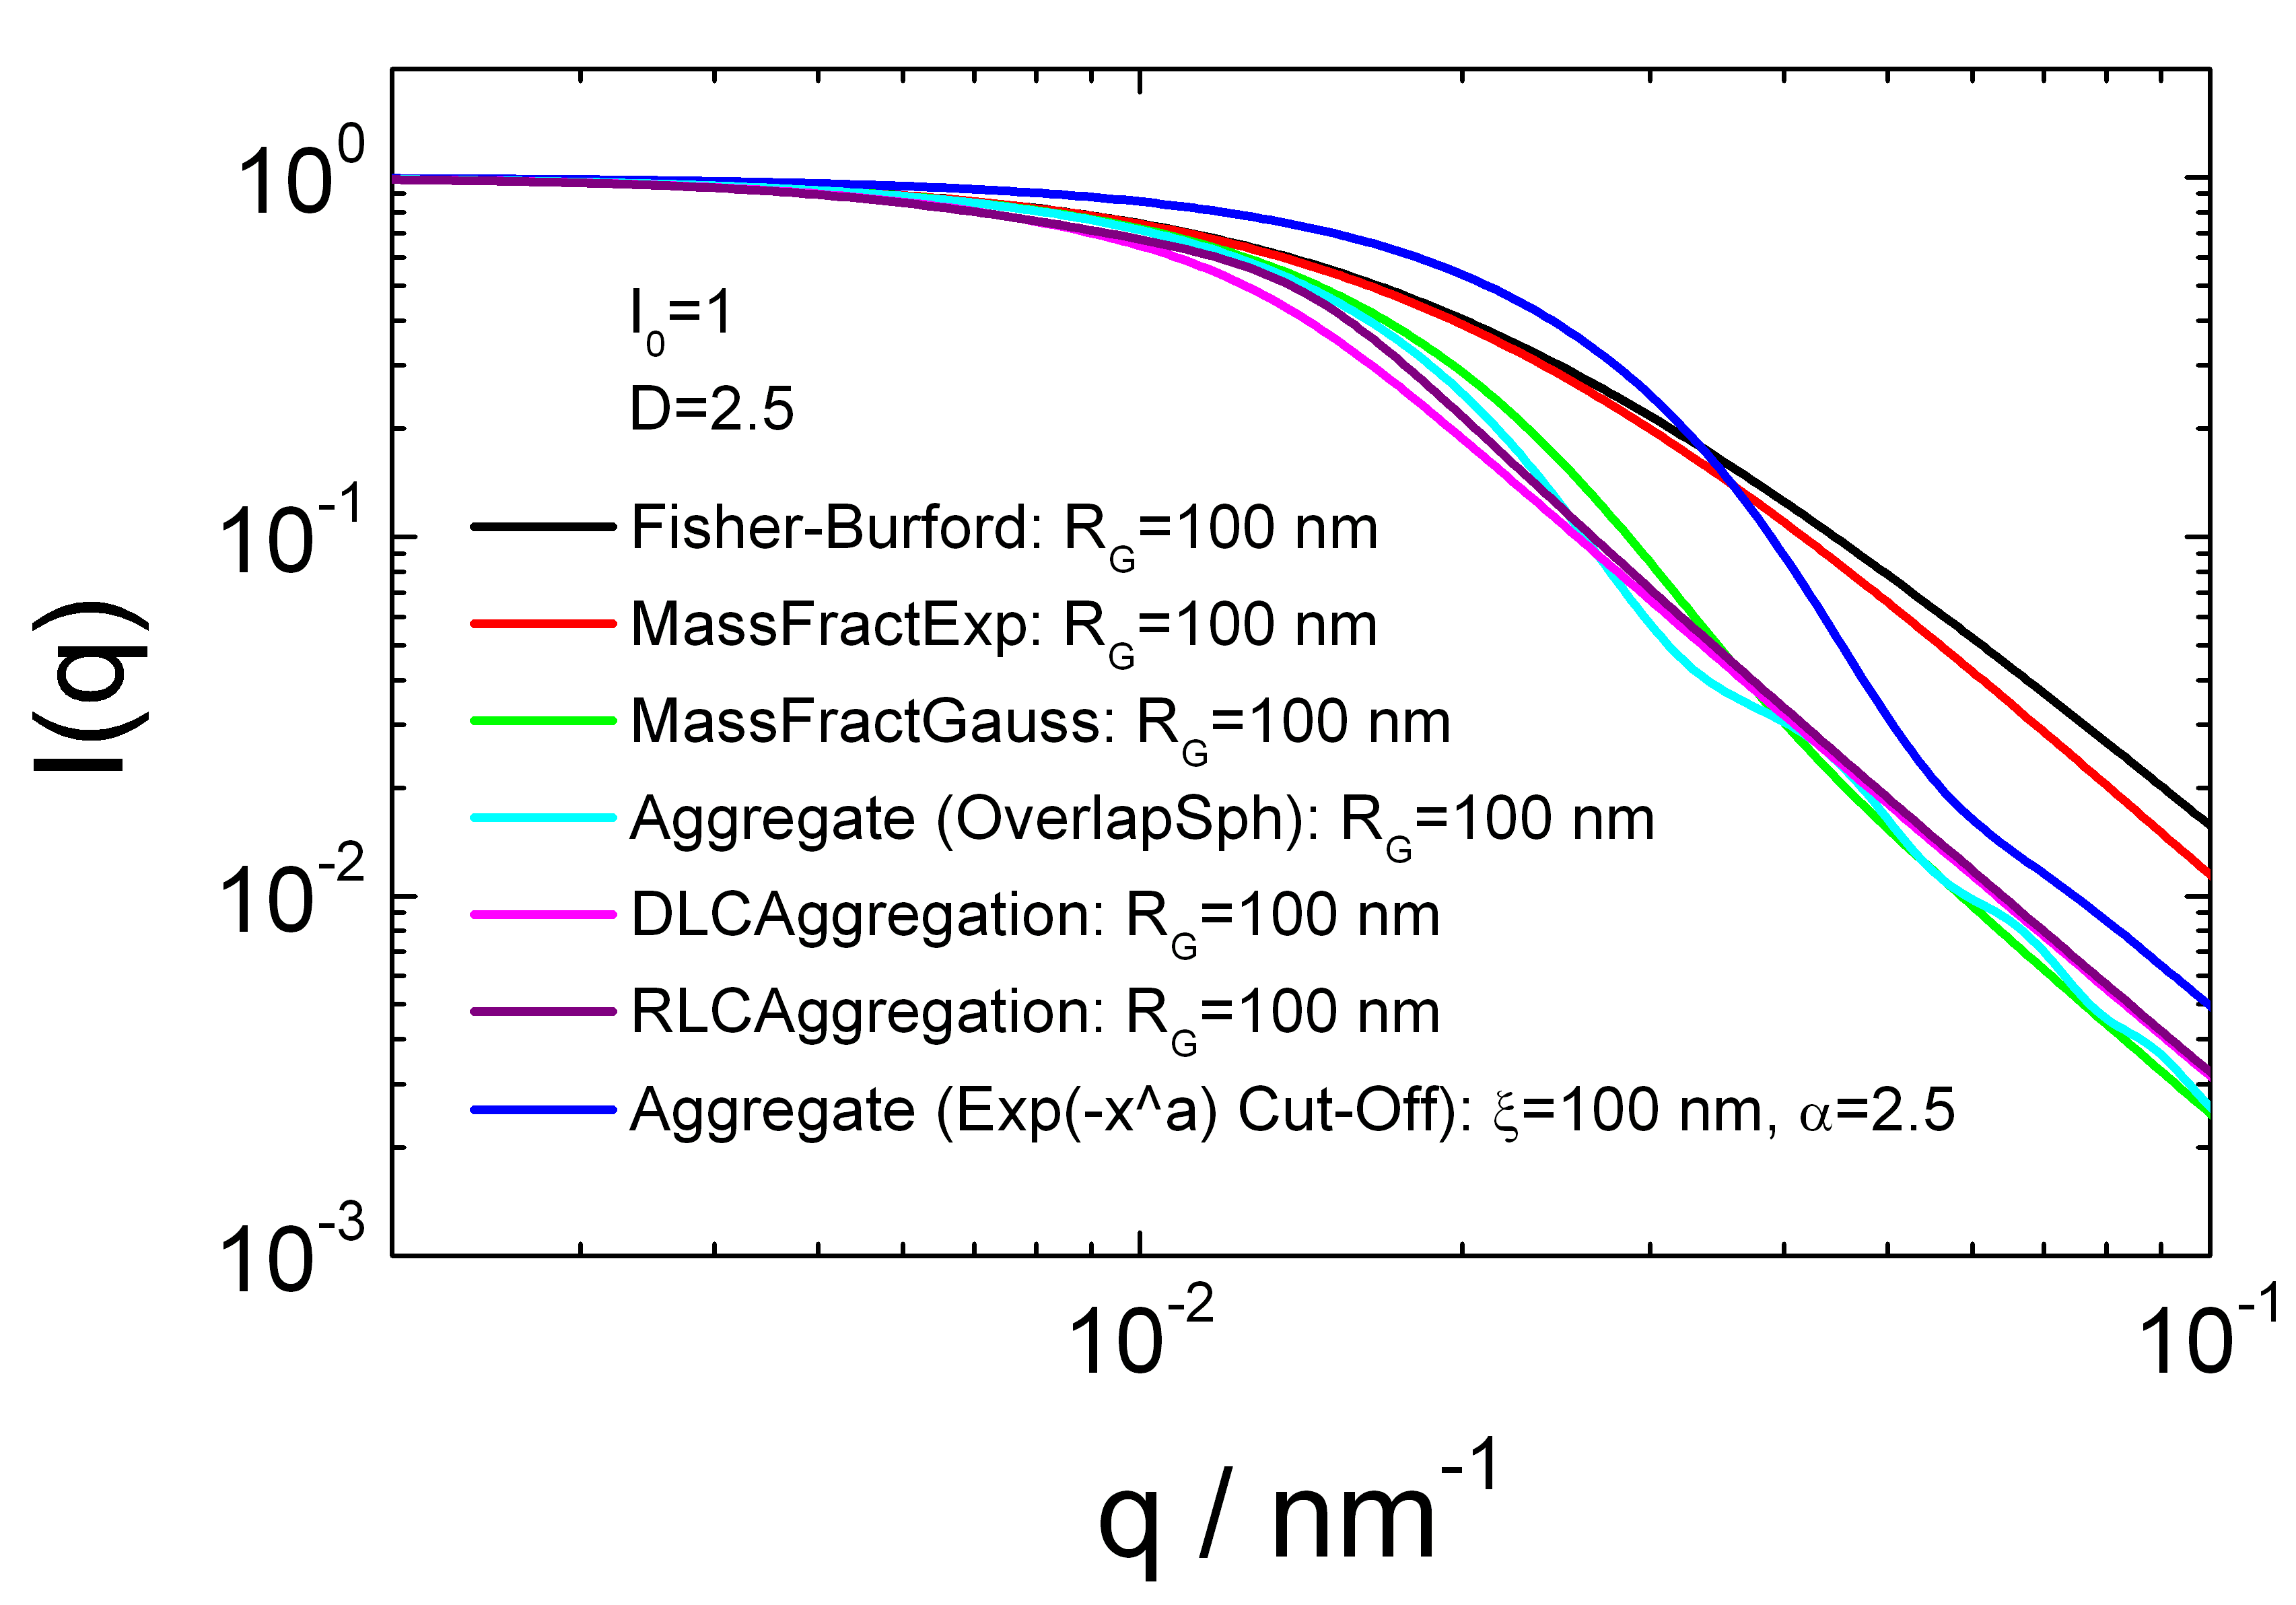
\includegraphics[width=0.768\textwidth,height=0.528\textwidth]{../images/form_factor/cluster/AggregateComparison.png}
\end{center}
\caption{Form factor for the different types of mass fractals listed in \ref{tab:SQ_cutuofffunctions}.}
\label{fig:FFCluster}
\end{figure}

%REFERENCES: ~\\
%\cite{Sorensen1999}
%1. C. M. Sorensen and G. M. Wang,
%Size distribution effect on the power law regime of the structure factor of fractal aggregates,
%Physical Review E, Vol 60, No. 6, (1999) 7143-7148 \\
%\cite{Sorensen1992}
%2. C. M. Sorensen, J. Cai, and N. Lu,
%Test of Static Structure Factors for Describing Light Scattering from Fractal Soot Aggregates,
%Langmuir 1992,8, 2064-2069\\
%\cite{Hurd1988}
%3. A.J. Hurd and W.L. Flower,
%In Situ Growth and Structure of Fractal Silica Aggregates in a Flame,
%Journal of Colloid and Interface Science, Vol. 122, No 1, (1988) 178--192 \\
%\cite{Lin1989}
%4. M.Y. Lin, H.M. Lindsay, D.A. Weitz, R.C. Ball, R. Klein, P. Meakin,
%Universality of Fractal Aggregates as Probed by Light Scattering,
%Proc. R. Soc. Lond. A \textbf{423}, 71-87 (1989) \\
%\cite{Lin1990}
%5. M.Y. Lin, H.M. Lindsay, D.A. Weitz, R.C. Ball, R. Klein, P. Meakin,
%Universal reaction-limited colloidal aggregation,
%Physical Review A, Vol 41, No. 4, 2005--2020 (1990) \\
%\cite{Lin1990a}
%5. M.Y. Lin, H.M. Lindsay, D.A. Weitz, R.C. Ball, R. Klein, P. Meakin,
%Universal diffusion-limited colloid aggregation
%J. Phys.: Condens. Matter 2 (1990) 3093-3113. \\

%\begin{align}
%I_\text{MassFract}(Q,\xi,D,R) =  \left(1 +  \cfrac{D \Gamma(D-1)
%\sin\left([D-1]\arctan(Q \xi)\right)}{\left( Q R\right)^D
%\left[1+\cfrac{1}{Q^2\xi^2}\right]^{(D-1)/2}}
%       \right) K^2(Q,R,\Delta\eta)
%\end{align}
%where $D$ is the fractal dimension, $\xi$ is a cut-off length for
%the fractal correlations, $\Gamma(x)$ is the gamma function, and
%$K^2(Q,R,\Delta\eta)$ the form factor of a sphere out of which the
%fractal consists.


%%%%%%%%%%%%%%%%%%%%%%%%%%%%%%%%%%%%%%%%%%%%%%%%%%%%%%%%%%%%%%%%%%


\clearpage
\subsection{Stacked Discs \cite{Kratky194935,Hanley2003}}
\label{sect:StackedDiscs}
~\\

\begin{figure}[htb]
\begin{center}
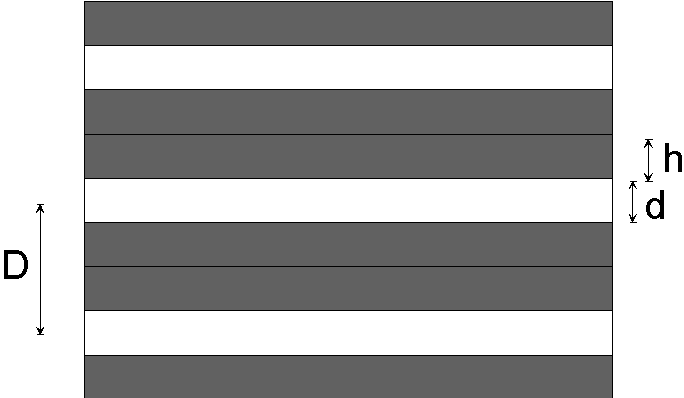
\includegraphics[width=0.5\textwidth,height=0.2908\textwidth]{../images/form_factor/cluster/stackdiscs.png}
\end{center}
\caption{Sketch for a stack of discs with an additional surface layer}
\label{stackeddiscs}
\end{figure}



\begin{align}
I_\text{StackedDiscs}(Q,R)&= \int_0^{\pi/2}\left( \Delta\eta_l
\left(V_t f_t - V_c f_c\right) + \Delta\eta_c  V_c f_c \right)^2
S(Q,\Theta) \sin(\Theta)\, d\Theta
\end{align}
Here it is assume that the nearest neighbor distance between the
platelets obeys a Gaussian distribution and consider an internal
structure factor, $S(Q,\Theta)$, first proposed by Kratky and Porod
in 1949 \cite{Kratky194935}
\begin{align}
S(Q,\Theta) &=  1+\frac{2}{n} \sum_{k=1}^{n-1} (n-k)
\cos(kDQ\cos(\Theta))
     \exp\left(-\frac{k}{2}\left(Q\cos(\Theta) \sigma_D\right)^2\right) \\
f_t &= f_t = \frac{\sin\left(Q(\frac{d}{2}+h)\cos(\Theta)\right)}{Q(\frac{d}{2}+h)\cos(\Theta)} \,\,\,\,2\frac{J_1(QR\sin(\Theta))}{QR\sin(\Theta)} \\
f_c &= f_c = \frac{\sin\left(Q\frac{d}{2}\cos(\Theta)\right)}{Q\frac{d}{2}\cos(\Theta)} \,\,\,\,2\frac{J_1(QR\sin(\Theta))}{QR\sin(\Theta)}\\
V_t &= \pi R^2 (d+2h)\\
V_c &= \pi R^2 d
\end{align}


\begin{figure}[htb]
\begin{center}
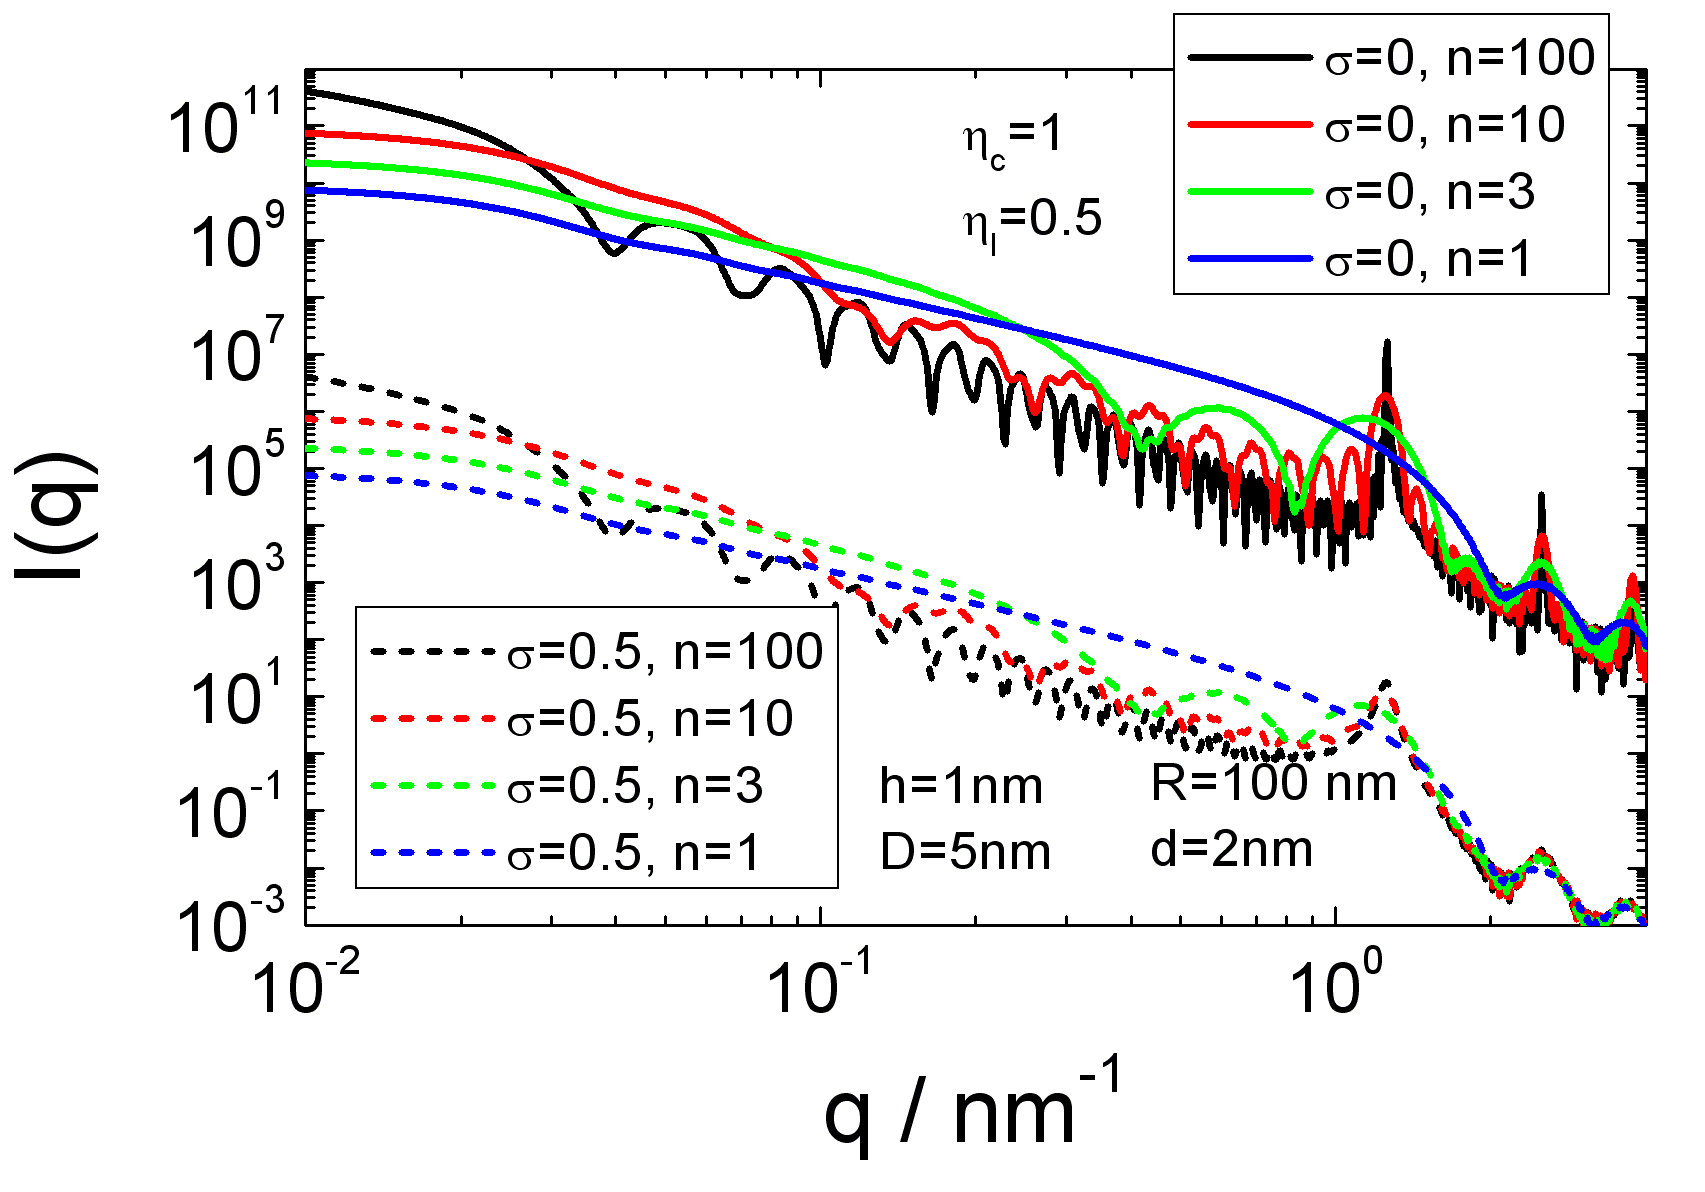
\includegraphics[width=0.768\textwidth,height=0.528\textwidth]{../images/form_factor/cluster/StackedDiscsIQ.png}
\end{center}
\caption{Scattering Intensity for a stack of discs with a layer.}
\label{fig:StackedDiscs}
\end{figure}

%%%%%%%%%%%%%%%%%%%%%%%%%%%%%%%%%%%%%%%%%%%%%%%%%%%%%%%%%%%%%%%%%%%%%%

\clearpage
\subsection{DumbbellShell}
\label{sect:DumbbellShell}
~\\

\begin{figure}[htb]
\begin{center}
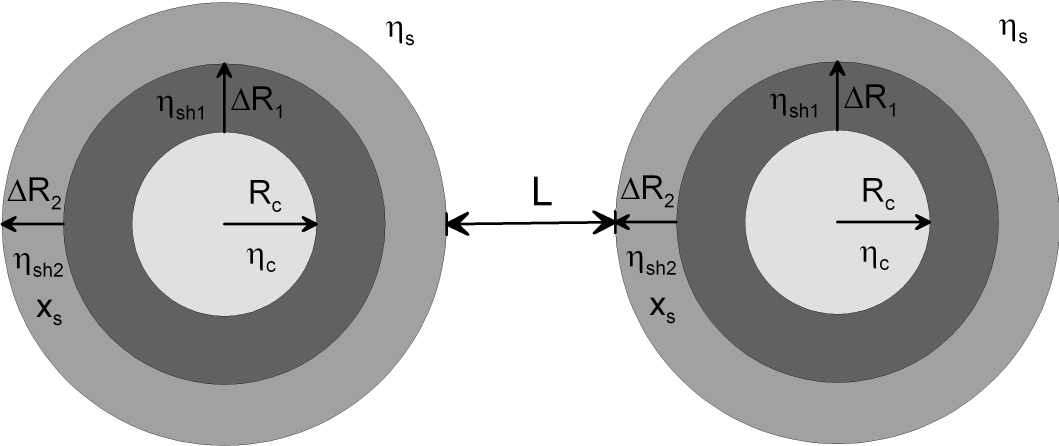
\includegraphics[width=0.8\textwidth,height=0.337\textwidth]{../images/form_factor/cluster/l_doubleshell.png}
%1059x446
\end{center}
\caption{} \label{DumbbellShell}
\end{figure}

%%%%%%%%%%%%%%%%%%%%%%%%%%%%%%%%%%%%%%%%%%%%%%%%%%%%%%%%%%%%%%%%%%%%%%%%%%%%%%%%%%%%%%

\clearpage
\subsection{DoubleShellChain}
\label{sect:DoubleShellChain}
~\\

\begin{figure}[htb]
\begin{center}
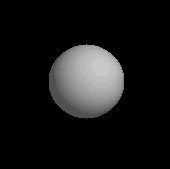
\includegraphics[width=0.18\textwidth,height=0.18\textwidth]{../images/form_factor/cluster/tetrahedron1.png}
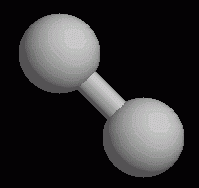
\includegraphics[width=0.18\textwidth,height=0.18\textwidth]{../images/form_factor/cluster/tetrahedron2.png}
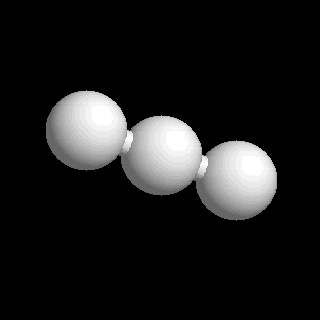
\includegraphics[width=0.18\textwidth,height=0.18\textwidth]{../images/form_factor/cluster/DoubleShellChain3.png}
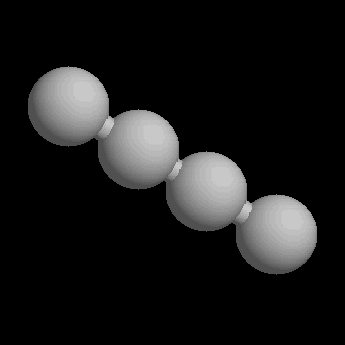
\includegraphics[width=0.18\textwidth,height=0.18\textwidth]{../images/form_factor/cluster/DoubleShellChain4.png}
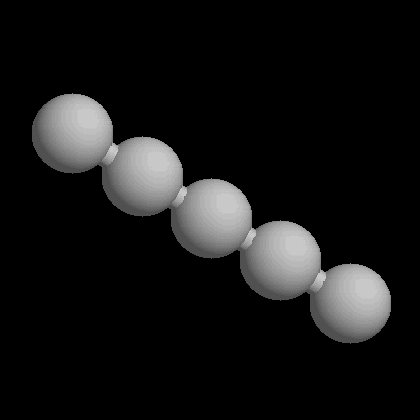
\includegraphics[width=0.18\textwidth,height=0.18\textwidth]{../images/form_factor/cluster/DoubleShellChain5.png}
\end{center}
\caption{} \label{doubleshellchain}
\end{figure}

\begin{figure}[htb]
\begin{center}
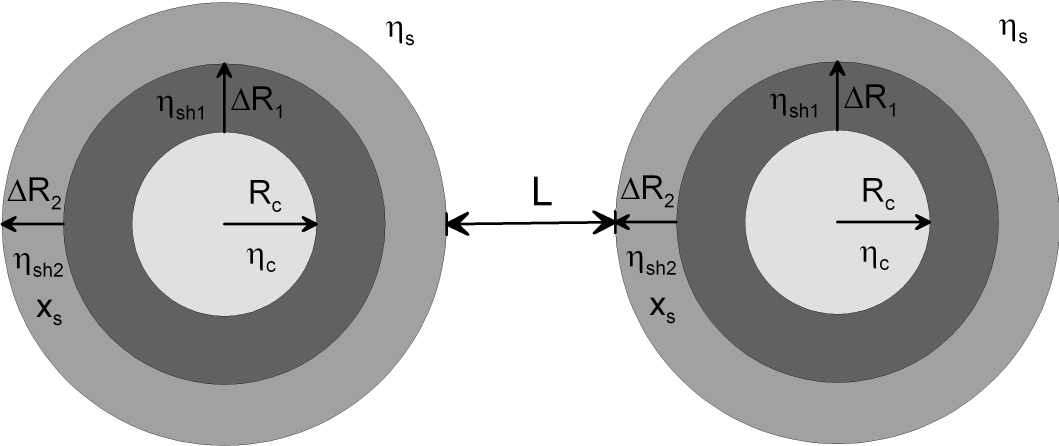
\includegraphics[width=0.8\textwidth,height=0.337\textwidth]{../images/form_factor/cluster/l_doubleshell.png}
%1059x446
\end{center}
\caption{} \label{doubleshell}
\end{figure}

\begin{figure}[htb]
\begin{center}
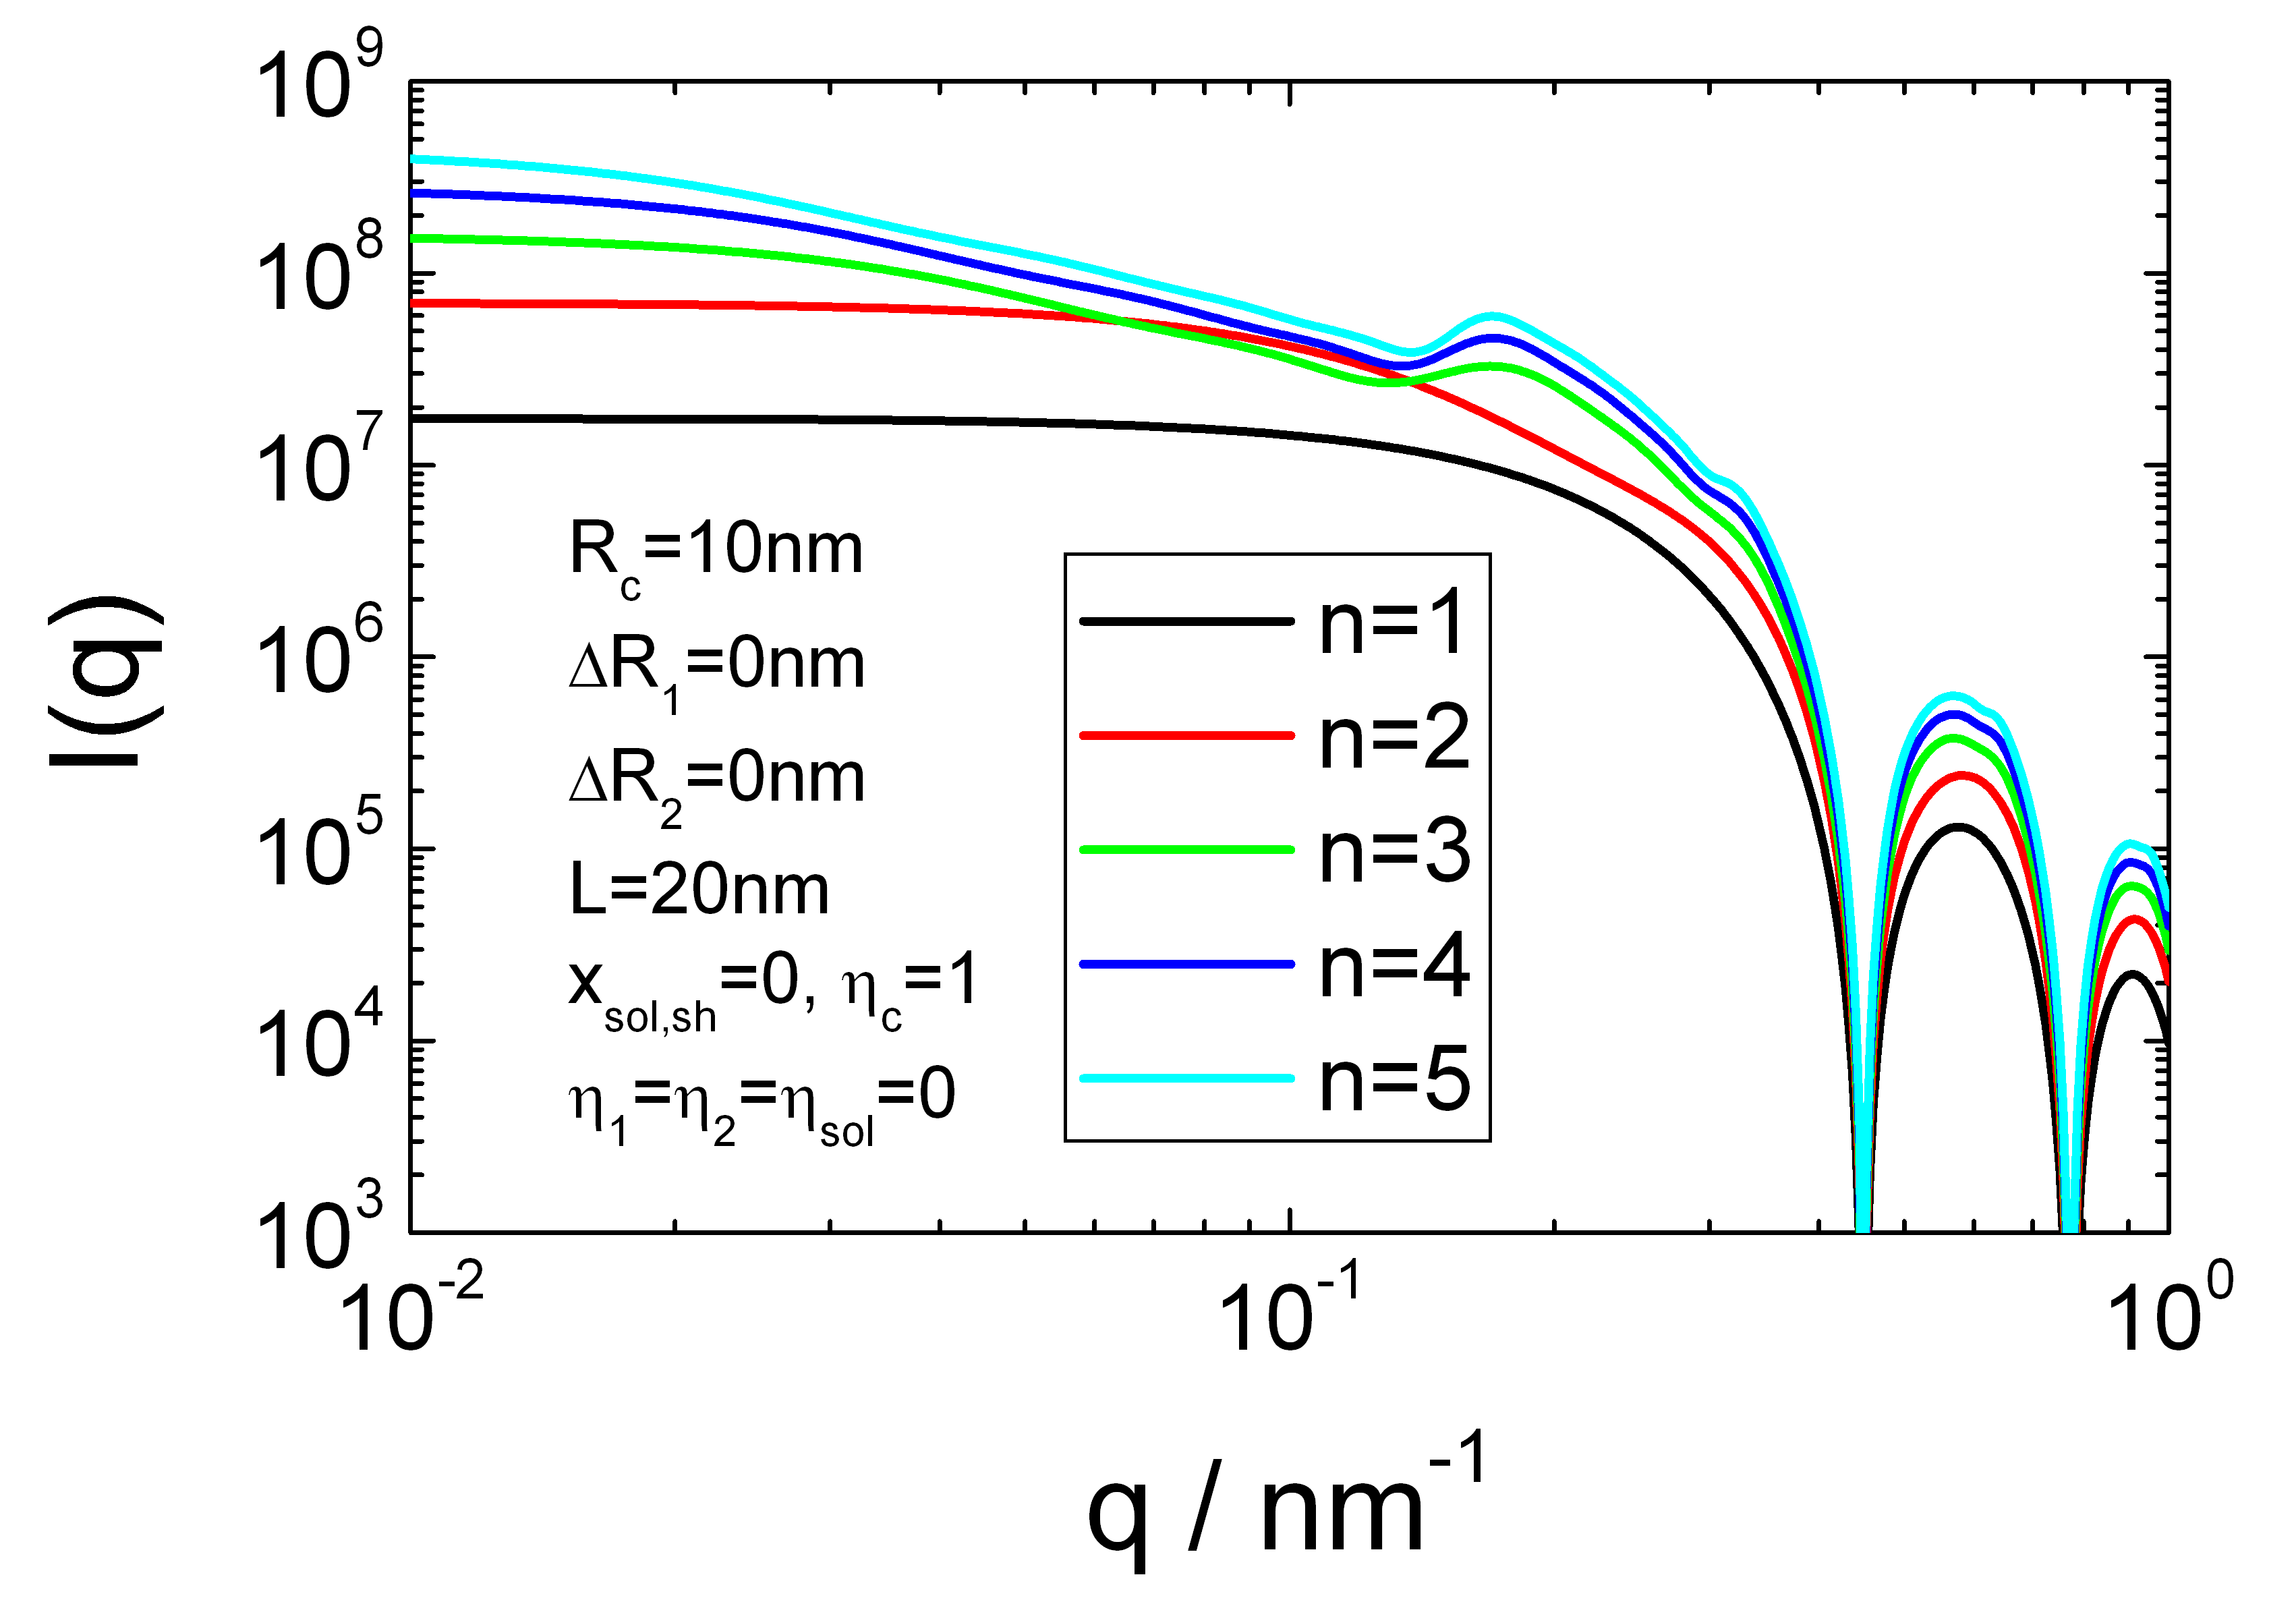
\includegraphics[width=0.8\textwidth,height=0.5\textwidth]{../images/form_factor/cluster/DoubleShellChain.png}
\end{center}
\caption{}
\label{fig:DoubleShellChain}
\end{figure}

%%%%%%%%%%%%%%%%%%%%%%%%%%%%%%%%%%%%%%%%%%%%%%%%%%%%%%%%%%%%%%%%%%%%%%%%%%%%%%

\clearpage
\subsection{TetrahedronDoubleShell}
\label{sect:TetrahedronDoubleShell}
~\\

\begin{figure}[htb]
\begin{center}
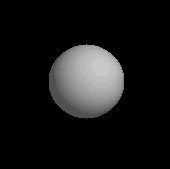
\includegraphics[width=0.18\textwidth,height=0.18\textwidth]{../images/form_factor/cluster/tetrahedron1.png}
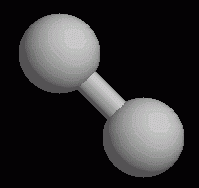
\includegraphics[width=0.18\textwidth,height=0.18\textwidth]{../images/form_factor/cluster/tetrahedron2.png}
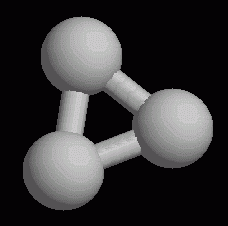
\includegraphics[width=0.18\textwidth,height=0.18\textwidth]{../images/form_factor/cluster/tetrahedron3.png}
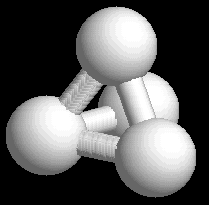
\includegraphics[width=0.18\textwidth,height=0.18\textwidth]{../images/form_factor/cluster/tetrahedron4.png}
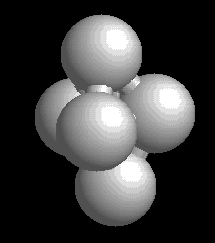
\includegraphics[width=0.18\textwidth,height=0.18\textwidth]{../images/form_factor/cluster/tetrahedron5.png}
\end{center}
\caption{} \label{tetrahedron}
\end{figure}
\begin{figure}[htb]
\begin{center}
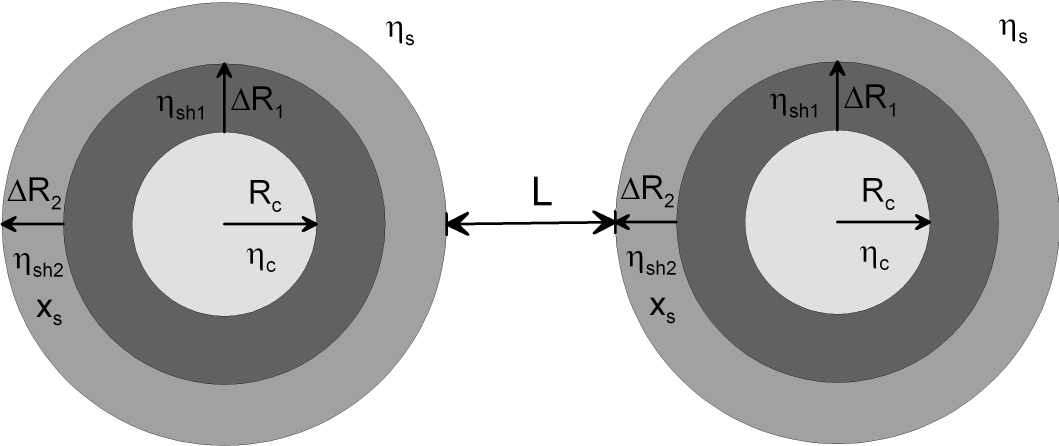
\includegraphics[width=0.8\textwidth,height=0.337\textwidth]{../images/form_factor/cluster/l_doubleshell.png}
%1059x446
\end{center}
\caption{}
\label{TetrahedronDoubleShell}
\end{figure}

\begin{figure}[htb]
\begin{center}
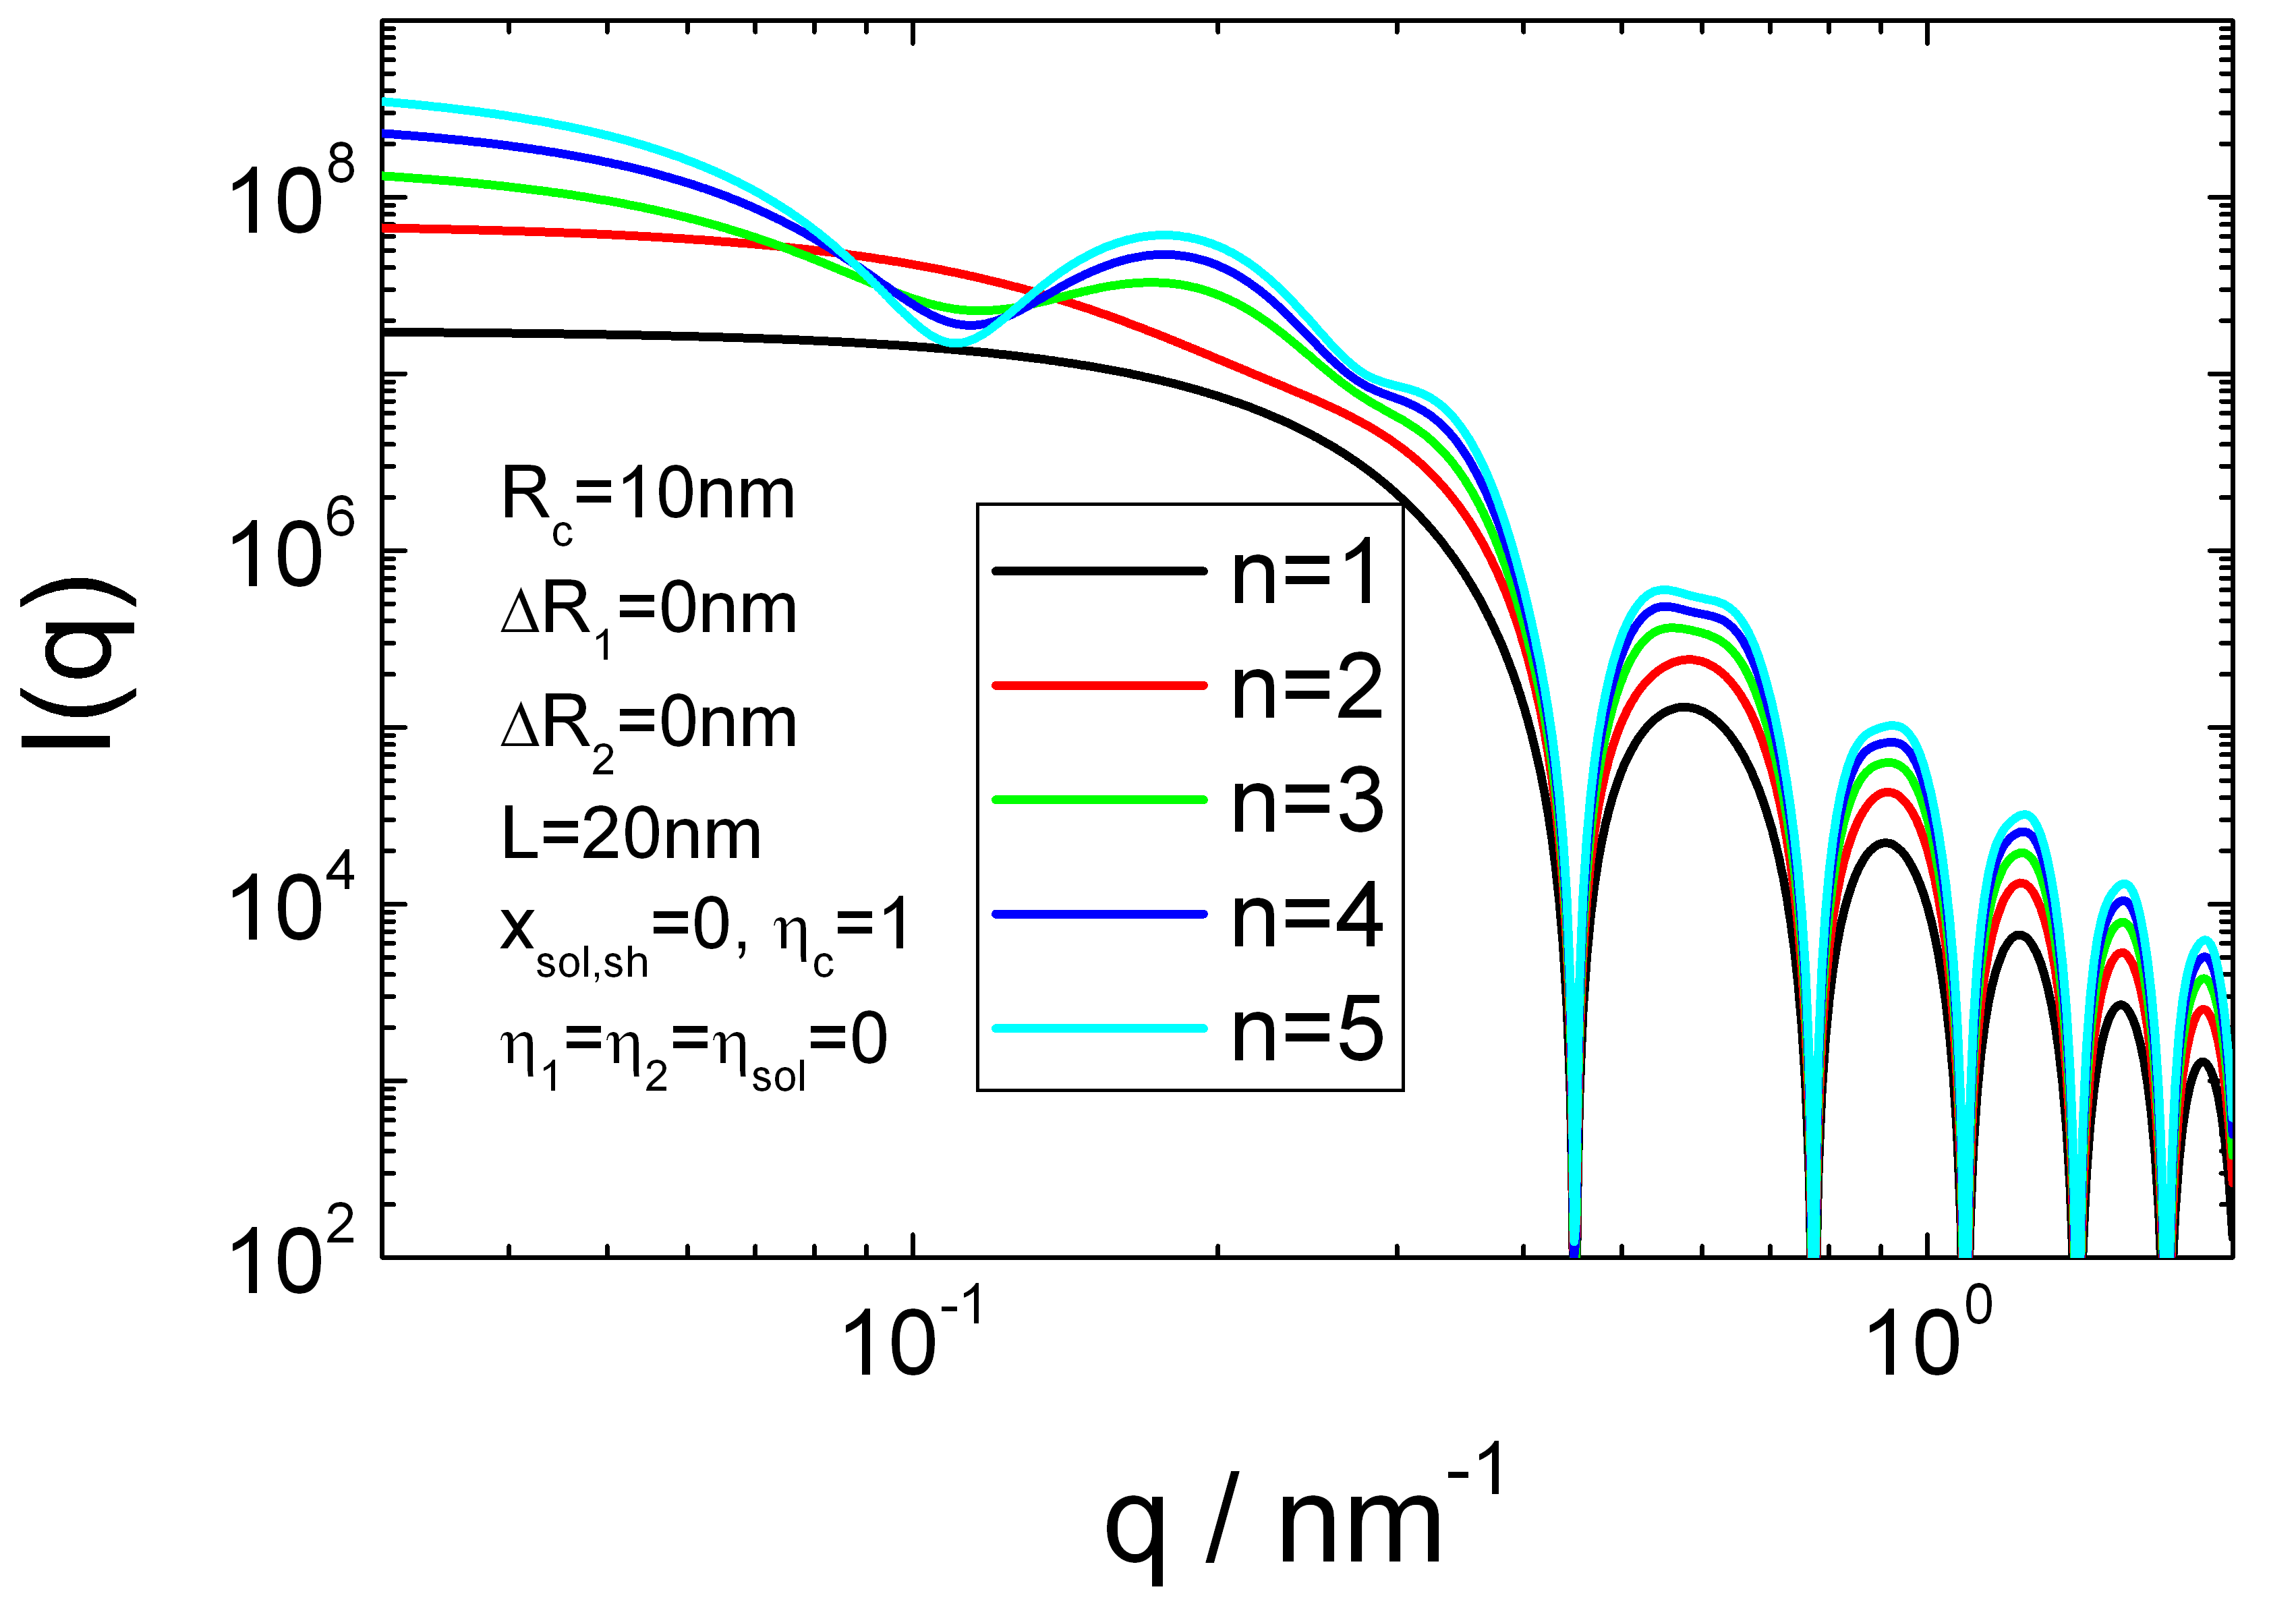
\includegraphics[width=0.8\textwidth,height=0.5\textwidth]{../images/form_factor/cluster/TetraHedronDoubleShell.png}
\end{center}
\caption{}
\label{fig:TetrahedronDoubleShell}
\end{figure}
